\documentclass{beamer}

\usepackage[utf8]{inputenc} 
\usepackage[T1]{fontenc}
\usepackage{lmodern}
\usepackage{graphicx}
\usepackage[english]{babel}

\usetheme{Frankfurt}

\title[Defense]{PROG1 Project 1}

\author{Simon Bihel, Florestan De Moor}
\institute[ENS Rennes]{
\includegraphics[scale=0.12]{ENS_Rennes.png}\\Computer Science Department, 1st year}
\date{October 9, 2015}

\begin{document}
	\begin{frame}
		\maketitle
	\end{frame}
	
	\begin{frame}
		\frametitle{Presentation of the project}
		\begin{columns}[T]
			\begin{column}{.5\textwidth}
				\hspace*{0cm} 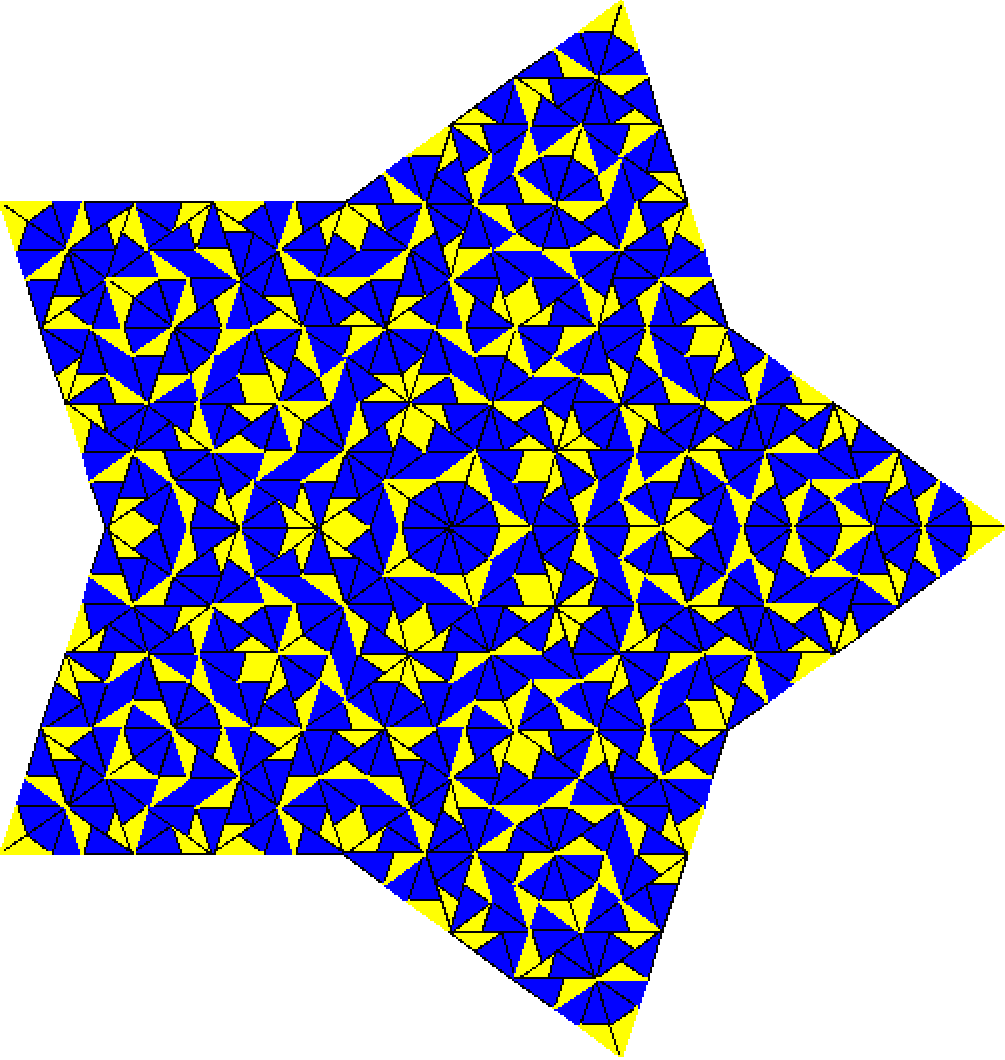
\includegraphics[height=0.65\textheight]{screenshot_star.png} \hspace*{\fill}
			\end{column}
			\begin{column}{.45\textwidth}
				\begin{itemize}
					\item Penrose tiling (Robinson triangles) ;
					\item Towers of Hanoi with n rodes and p disks.
				\end{itemize}
			\end{column}
		\end{columns}
	\end{frame}
	
	\begin{frame}
		\frametitle{Summary}
		\tableofcontents
	\end{frame}
	
	\section{Penrose}
	\subsection{Basic features}
	\begin{frame}
		\frametitle{Penrose tiling, basic features}
		\begin{itemize}
			\item Recursive division of Robinson triangles.
		\end{itemize}
	\end{frame}
	
	\subsection{Advenced features}
	\begin{frame}
		\frametitle{Advanced features}
		\begin{itemize}
			\item Wheel of triangles.
		\end{itemize}
	\end{frame}
	
	\section{Hanoi}
	\subsection{Basic features}
	\begin{frame}
		\frametitle{Tower of Hanoi, basic features}
	\end{frame}
	
	\section*{Conclusion}
	\begin{frame}
		\frametitle{Conclusion}
	\end{frame}

\end{document}
